\chapter{RESULTADOS}
\label{cap:resultados}

Este capítulo sigue la estructura del Capítulo~\ref{cap:metodo}: cada título lleva
entre corchetes el enlace a su sección homóloga del método, de modo que ambos
capítulos se corresponden uno a uno. Las tres unidades se ejecutaron:
preprocesamiento de los escaneos, extracción de descriptores y evaluación de
M2 a M4. Se distingue siempre entre la corrida de entrenamiento de HyperNCD, que
fue una, y las semillas posteriores del agrupamiento, que fueron diez.

% =====================================================================
\FloatBarrier
\section[Diagrama de Flujo General]{Diagrama de Flujo General\espejo{sec:diagrama-flujo}}
\label{sec:res-flujo}

De las etapas de la Figura~\ref{fig:flujo} se ejecutaron E0 a E5
(Tabla~\ref{tab:res-etapas}).

\begin{table}[!htbp]
\centering
\setstretch{1}\small
\caption[Etapas ejecutadas del flujo general]{Etapas ejecutadas del flujo general y dónde está su resultado. Elaboración propia.}
\label{tab:res-etapas}
\begin{tabularx}{\linewidth}{@{}l>{\raggedright\arraybackslash}X>{\raggedright\arraybackslash}X@{}}
\toprule
\textbf{Etapa} & \textbf{Alcance ejecutado} & \textbf{Resultado} \\
\midrule
E0. Preparación & 23 archivos LAS preprocesados; PL13, PL7 y la capilla etiquetada en detalle & \S\ref{sec:res-unidad1}, Tabla~\ref{tab:m1-metadatos} \\
E1. Diagnóstico de dominio & M2 entrenado con SemanticPOSS aplicado a la capilla & \S\ref{sec:res-u3-proc}, Tabla~\ref{tab:m2-control} \\
E2. Entrenamiento de M2 & Una corrida de 30 épocas con ArCH & \S\ref{sec:res-u3-proc}, Figura~\ref{fig:m2-arch-curvas} \\
E3. Inferencia congelada & $f_{\mathrm{sem}}$ de M2 y $f_{\mathrm{ssl}}$ de Sonata, escritos a disco & \S\ref{sec:res-unidad2}, Tabla~\ref{tab:salidas-p2} \\
E4. Fusión y agrupamiento & M2, M3, M4 base y M4 con $K=8$ & \S\ref{sec:res-u3-rep}, Tabla~\ref{tab:m2-m4-semillas} \\
E5. Evaluación & mIoU uno a uno, NMI, ARI y IoU por clase, con diez semillas & \S\ref{sec:res-u3-traza}, Figura~\ref{fig:m4-semillas} \\
\bottomrule
\end{tabularx}
\end{table}

La frontera de disco funciona en ambos sentidos: las ramas congeladas escriben
sus descriptores y la etapa de fusión los lee sin mantener a la vez en memoria
los entornos de HyperNCD y Sonata.

% =====================================================================
\FloatBarrier
\section[Hardware y Repositorio]{Hardware y Repositorio\espejo{sec:hardware-repo}}
\label{sec:res-hardware}

Cada etapa corrió en el equipo que indica la Tabla~\ref{tab:res-hardware}, con
los programas y guiones del repositorio y las órdenes del
\hyperref[sec:anexo-software]{Anexo~A}. La memoria de GPU de la fila de M2 es la
que informa \texttt{nvidia-smi}; el pico que registra PyTorch para esa misma
extracción es menor, 3{,}2\,GB, porque no cuenta el contexto de CUDA.

\begin{table}[!htbp]
\centering
\setstretch{1}\small
\caption[Equipo, tiempo y memoria de cada etapa]{Equipo, tiempo y memoria de cada etapa ejecutada. Elaboración propia a partir de los registros de medición.}
\label{tab:res-hardware}
\begin{tabularx}{\linewidth}{@{}>{\raggedright\arraybackslash}Xlrr@{}}
\toprule
\textbf{Etapa} & \textbf{Equipo} & \textbf{Tiempo} & \textbf{Memoria pico} \\
\midrule
M1, PL13 y PL7 & Laptop local & 12{,}0 y 14{,}4\,s & --- \\
M1, 23 archivos & Khipu, CPU & 1\,079\,s en total & --- \\
Sonata, PL13 & Khipu, RTX A6000 & 13{,}9\,s & 34{,}60\,GB \\
Entrenamiento de M2, ArCH & Colab, T4 & 75{,}0\,min & 9{,}5\,GB (GPU); 4{,}91\,GB (RAM) \\
M2 sobre la capilla & Colab, T4 & 42{,}7\,s & 5{,}28\,GB (GPU); 4{,}49\,GB (RAM) \\
Sonata, capilla & Colab, L4 & 26{,}6\,s & 10{,}49\,GB \\
M4, capilla & CPU local & 68 a 80\,s & --- \\
\bottomrule
\end{tabularx}
\end{table}

% =====================================================================
\FloatBarrier
\section[Diseño General del Sistema]{Diseño General del Sistema\espejo{sec:diseno}}
\label{sec:res-diseno}

\FloatBarrier
\subsection[Estructura y Contrato de los Módulos]{Estructura y Contrato de los Módulos\espejo{sec:contrato}}
\label{sec:res-contrato}

El contrato de la Tabla~\ref{tab:contrato} es el diseño; la
Tabla~\ref{tab:res-contrato} indica qué se ejecutó de cada módulo. La diferencia
principal es que M2 y M4 no se ejecutaron como módulos entrenados dentro del
mismo ciclo: M2 se entrenó antes y se aplicó congelado, y M4 operó después, sobre
los descriptores guardados.

\begin{table}[!htbp]
\centering
\setstretch{1}\small
\caption[Contrato de diseño frente a ejecución]{Contrato de cada módulo frente a lo ejecutado. Elaboración propia.}
\label{tab:res-contrato}
\begin{tabularx}{\linewidth}{@{}l>{\raggedright\arraybackslash}X>{\raggedright\arraybackslash}X@{}}
\toprule
\textbf{Módulo} & \textbf{Salida del contrato} & \textbf{Ejecutado} \\
\midrule
M1 & Matriz $S$ de 9 columnas (Tabla~\ref{tab:m1-metadatos}) & 23 archivos; PL13, PL7 y la capilla verificados \\
M2 & $f_{\mathrm{sem}}$ de 96 dimensiones, logits e índice inverso & Entrenado con SemanticPOSS y con ArCH; extraído una vez por escena con el checkpoint congelado \\
M3 & $f_{\mathrm{ssl}}$ de 1088 valores con índice inverso (Tabla~\ref{tab:npz}) & Sonata congelado, original y adaptado, una vez por escena \\
M4 & Etiqueta $\hat{y}_i$ por punto & Fusión posterior en CPU: regiones de 0{,}75\,m, afinidad, hiperaristas y prototipos con Sinkhorn--Knopp; sin gradientes \\
M5 & Métricas y visor & mIoU uno a uno, NMI, ARI, IoU por clase y visor 3D \\
\bottomrule
\end{tabularx}
\end{table}

\FloatBarrier
\subsection[Visor 3D del Proyecto]{Visor 3D del Proyecto\espejo{sec:visor}}
\label{sec:res-visor}

Al dibujar los descriptores de PL13 (Figura~\ref{fig:visor-pl13-etapas}), el
visor verificó que el archivo \texttt{.npz} corresponde a la matriz $S$ de la que
salió. Con la capilla etiquetada, el mismo visor produjo los mapas de clases y de
cabezas de M2 usados en este capítulo.

% =====================================================================
\FloatBarrier
\section[Unidad 1. Preprocesamiento]{Unidad 1. Preprocesamiento\espejo{sec:unidad1}}
\label{sec:res-unidad1}

\FloatBarrier
\subsection[Datos de Entrada y Ejecución]{Datos de Entrada y Ejecución\espejo{sec:u1-datos}}
\label{sec:res-u1-datos}

El procedimiento se ejecutó sobre dos escaneos de la Catedral de Lima, PL13 y
PL7, en el equipo local de la Sección~\ref{sec:hardware-repo}. PL13 es el
escaneo principal, porque es el que después pasa por Sonata en la
Sección~\ref{sec:res-unidad2}, de modo que todo el análisis sigue al mismo
escaneo de principio a fin. PL7 se presenta al lado como segundo ejemplo, para
mostrar que el procedimiento se comporta igual en otro escaneo. PL13 es el
1{,}40\,\% del levantamiento y PL7 el 1{,}46\,\%.

Las dos pruebas usaron los valores por defecto de la
Sección~\ref{sec:u1-procedimiento} (Tabla~\ref{tab:m1-metadatos}).
Las figuras de nubes de esta sección dibujan 200\,000 puntos tomados al azar,
salvo donde se indique.


\paragraph*{Escena de control.} Para medir con etiquetas se usó una capilla de la
Catedral anotada con cinco clases (arco, columna, cúpula, pared y techo) más
\emph{otro}. El Módulo~1 la redujo de 3\,380\,661 puntos a 3\,277\,440 tras el
filtrado (3{,}1\,\%) y a 1\,135\,946 tras la voxelización, en 9{,}3\,s; las
etiquetas se transfirieron con una distancia mediana de 1{,}2\,cm y máxima de
3{,}6\,cm. La Tabla~\ref{tab:capilla-clases} muestra que el vóxel conserva entre
31 y 36\,\% de cada clase, de modo que no sesga su proporción.

\begin{table}[!htbp]
\centering
\setstretch{1}\small
\caption[Clases de la escena de control antes y después del Módulo 1]{Puntos por clase de la capilla etiquetada antes y después del Módulo~1. Elaboración propia.}
\label{tab:capilla-clases}
\begin{tabular}{@{}lrrrr@{}}
\toprule
\textbf{Clase} & \textbf{Crudos} & \textbf{Tras M1} & \textbf{Conservado} & \textbf{Parte tras M1} \\
\midrule
Arco & 145\,927 & 47\,789 & 32{,}7\,\% & 4{,}2\,\% \\
Columna & 107\,105 & 33\,278 & 31{,}1\,\% & 2{,}9\,\% \\
Cúpula & 307\,330 & 110\,152 & 35{,}8\,\% & 9{,}7\,\% \\
Pared & 527\,591 & 173\,886 & 33{,}0\,\% & 15{,}3\,\% \\
Techo & 226\,478 & 75\,056 & 33{,}1\,\% & 6{,}6\,\% \\
Otro & 2\,066\,230 & 695\,785 & 33{,}7\,\% & 61{,}3\,\% \\
\bottomrule
\end{tabular}
\end{table}

\FloatBarrier
\subsection[Procedimiento]{Procedimiento\espejo{sec:u1-procedimiento}}
\label{sec:res-u1-procedimiento}

Los seis pasos se ejecutaron como los define la
Sección~\ref{sec:u1-procedimiento}; su evidencia visual, paso a paso y para los
dos escaneos, está en el \hyperref[sec:anexo-evidencia-m1]{Anexo~E}. En
resumen: la carga leyó cada escaneo en dos bloques en cerca de un segundo; el
centrado dejó cada nube en su propio origen; el filtrado SOR descartó el
2{,}66\,\% de los puntos de PL13 y el 4{,}73\,\% de PL7, concentrados en las
zonas ralas; la voxelización dejó como representantes el 10{,}01\,\% y el
7{,}46\,\% de los puntos filtrados; y las normales toman el mismo tono en las
superficies con la misma orientación, con manchas en las mismas zonas ralas que
concentraron los descartes del filtrado.

La escritura final dejó la matriz $S$ de PL13 en 28{,}9\,MB y la de PL7 en
22{,}0\,MB, cada una junto a su archivo de metadatos
(Tabla~\ref{tab:m1-metadatos}).

\begin{table}[!htbp]
\centering
\setstretch{1}\small
\caption[Metadatos de PL13 y PL7]{Metadatos de PL13 y PL7. Los campos se describen en el Paso~6 de la Sección~\ref{sec:u1-procedimiento}. Elaboración propia.}
\label{tab:m1-metadatos}
\begin{tabularx}{\linewidth}{@{}l>{\raggedright\arraybackslash}X>{\raggedright\arraybackslash}X@{}}
\toprule
\textbf{Campo} & \textbf{PL13} & \textbf{PL7} \\
\midrule
\texttt{voxel} & 0{,}05 & 0{,}05 \\
\texttt{q} & 20 & 20 \\
\texttt{lambda} & 2 & 2 \\
\texttt{offset\_utm} & \multicolumn{2}{l}{Columna \emph{Centro} de la Tabla~\ref{tab:m1-centrado}} \\
\texttt{n\_crudo} & 8\,239\,904 & 8\,590\,904 \\
\texttt{n\_sor} & 8\,020\,796 & 8\,184\,419 \\
\texttt{n\_voxel} & 803\,099 & 610\,637 \\
\texttt{segundos} & 12{,}0 & 14{,}4 \\
\bottomrule
\end{tabularx}
\end{table}

\FloatBarrier
\subsection[Verificación y Reproducibilidad]{Verificación y Reproducibilidad\espejo{sec:u1-reproducibilidad}}
\label{sec:res-u1-repro}

PL13 se ejecutó con la orden de la Sección~\ref{sec:u1-reproducibilidad} y PL7
con la siguiente.
\begin{lstlisting}[style=comando]
python preprocesar.py --input PL7_SCN0001.las \
       --output PL7_SCN0001_preprocesado \
       --voxel 0.05 --q 20 --lam 2
\end{lstlisting}

El mismo programa preprocesó después el levantamiento completo en el clúster
Khipu, con los mismos parámetros. Los 23 archivos LAS
(Sección~\ref{sec:u1-datos}) quedaron en 17\,807\,859 representantes. La suma de los tiempos por
archivo fue de 1\,079 segundos, unos 18 minutos. Los conteos de PL13 y de PL7
en esa corrida coinciden exactamente con los de las pruebas locales de la
Tabla~\ref{tab:m1-metadatos}, que es la comprobación de repetición descrita en
la Sección~\ref{sec:u1-reproducibilidad}: la unidad da el mismo resultado en dos
máquinas distintas.

% =====================================================================
\FloatBarrier
\section[Unidad 2. Extracción de Descriptores y Fusión]{Unidad 2. Extracción de Descriptores y Fusión\espejo{sec:unidad2}}
\label{sec:res-unidad2}

\FloatBarrier
\subsection[Rama Semántica]{Rama Semántica\espejo{sec:rama-sem}}
\label{sec:res-rama-sem}

La rama se ejecutó dos veces sobre la capilla con el mismo programa, una con el
checkpoint de SemanticPOSS y otra con el de ArCH, siempre congelada. Cada
ejecución produjo $f_{\mathrm{sem}}$ de 96 dimensiones, las puntuaciones de las
cabezas y el índice inverso, en 42{,}7\,s sobre una GPU T4 con ArCH
(Sección~\ref{sec:res-entorno}). La Tabla~\ref{tab:m2-novedoso} resume cómo se
comporta cada checkpoint como clasificador punto a punto, antes de cualquier
fusión. Con SemanticPOSS, M2 marca como novedoso el 99{,}1\,\% de la escena y casi
todas las clases reales, incluida la pared, caen en una sola cabeza; con ArCH solo
se marca el 12{,}6\,\% y la proporción depende de la clase: el arco, la clase más
ajena a lo conocido, se marca en 58{,}0\,\% y la pared en 1{,}0\,\%. El mIoU uno a
uno de las cabezas sin \emph{otro} pasa de 0{,}093 a 0{,}426.

\begin{table}[!htbp]
\centering
\setstretch{1}\small
\caption[M2 como clasificador punto a punto en la capilla]{Cabezas de M2 usadas como clasificador punto a punto en la capilla, sin fusión. Elaboración propia a partir de los registros del repositorio.}
\label{tab:m2-novedoso}
\begin{tabular}{@{}lrr@{}}
\toprule
\textbf{Medida} & \textbf{SemanticPOSS} & \textbf{ArCH} \\
\midrule
Puntos marcados como novedosos & 99{,}1\,\% & 12{,}6\,\% \\
Rango efectivo de $f_{\mathrm{sem}}$ & 3{,}4 & 1{,}7 \\
mIoU por mayoría, sin \emph{other} & 0{,}094 & 0{,}442 \\
mIoU uno a uno, sin \emph{other} & 0{,}093 & 0{,}426 \\
Arco marcado como novedoso & 99{,}9\,\% & 58{,}0\,\% \\
Pared marcada como novedosa & 98{,}9\,\% & 1{,}0\,\% \\
\bottomrule
\end{tabular}
\end{table}

El rango efectivo bajo no es señal de colapso: en SemanticPOSS también es bajo
(entre 4 y 5) donde el modelo funciona. Lo que delata el colapso es el reparto de
cabezas y el NMI (Sección~\ref{sec:res-u3-proc}).

\FloatBarrier
\subsection[Rama Auto-supervisada Congelada]{Rama Auto-supervisada Congelada\espejo{sec:rama-ssl}}
\label{sec:res-rama-ssl}

Se ejecutó sobre PL13 en Khipu. En el clúster
el archivo se llama \texttt{PL13'\_SCN0001.las}, con apóstrofo, y el guion de
lanzamiento lo quita al nombrar la salida, que queda como
\texttt{PL13\_SCN0001}. La entrada fue la matriz $S$ de PL13 generada en Khipu
(Sección~\ref{sec:res-u1-repro}), en 15{,}8 segundos.


\FloatBarrier
\subsubsection*{Paso 1. Carga de la matriz}

Se leen 803\,099 filas en 0{,}3 segundos; es la salida del Paso~6 de la
Unidad~1 (Figura~\ref{fig:m3-paso1}).

\begin{figure}[!htbp]
\centering
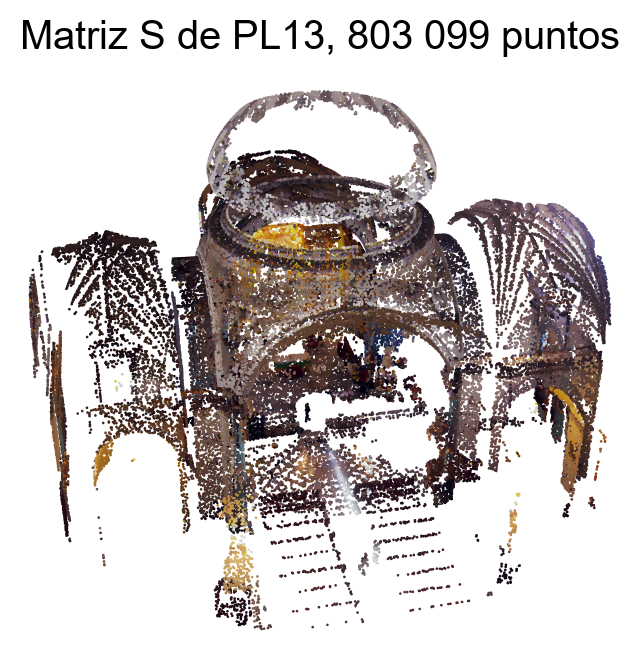
\includegraphics[width=0.4\linewidth]{imagenes/m3_paso1_entrada.png}
\caption[Matriz $S$ de PL13, entrada de Sonata]{Matriz $S$ de PL13, entrada de Sonata. Elaboración propia con el visor del proyecto (\hyperref[sec:anexo-software]{Anexo~A}).}
\label{fig:m3-paso1}
\end{figure}

\FloatBarrier
\subsubsection*{Paso 2. Carga del modelo}

El modelo cargado tiene 108{,}46 millones de parámetros, cifra que imprime la
función de carga de Sonata.

\FloatBarrier
\subsubsection*{Paso 3. Preparación}

La rejilla retiene casi todos los puntos (Tabla~\ref{tab:salidas-p2}). La
diferencia no se distingue a simple vista, por eso este paso no lleva imagen. La
causa es que el vóxel de 5\,cm de la
Unidad~1 ya dejó la nube más gruesa que la rejilla de Sonata, de modo que casi
toda celda contiene un solo punto.

\FloatBarrier
\subsubsection*{Paso 4. Inferencia}

El tiempo, el rendimiento y la memoria de la inferencia están en la
Tabla~\ref{tab:salidas-p2}. La Figura~\ref{fig:visor-pl13-etapas} muestra los
descriptores con la primera vista de la Sección~\ref{sec:revision-descriptores}.
Cada panel dibuja 100\,000 puntos al azar, por eso la
reducción de la Unidad~1 no se aprecia entre los dos primeros; se aprecia en la
Figura~\ref{fig:m1-paso4-pl13}.

\begin{figure}[!htbp]
\centering
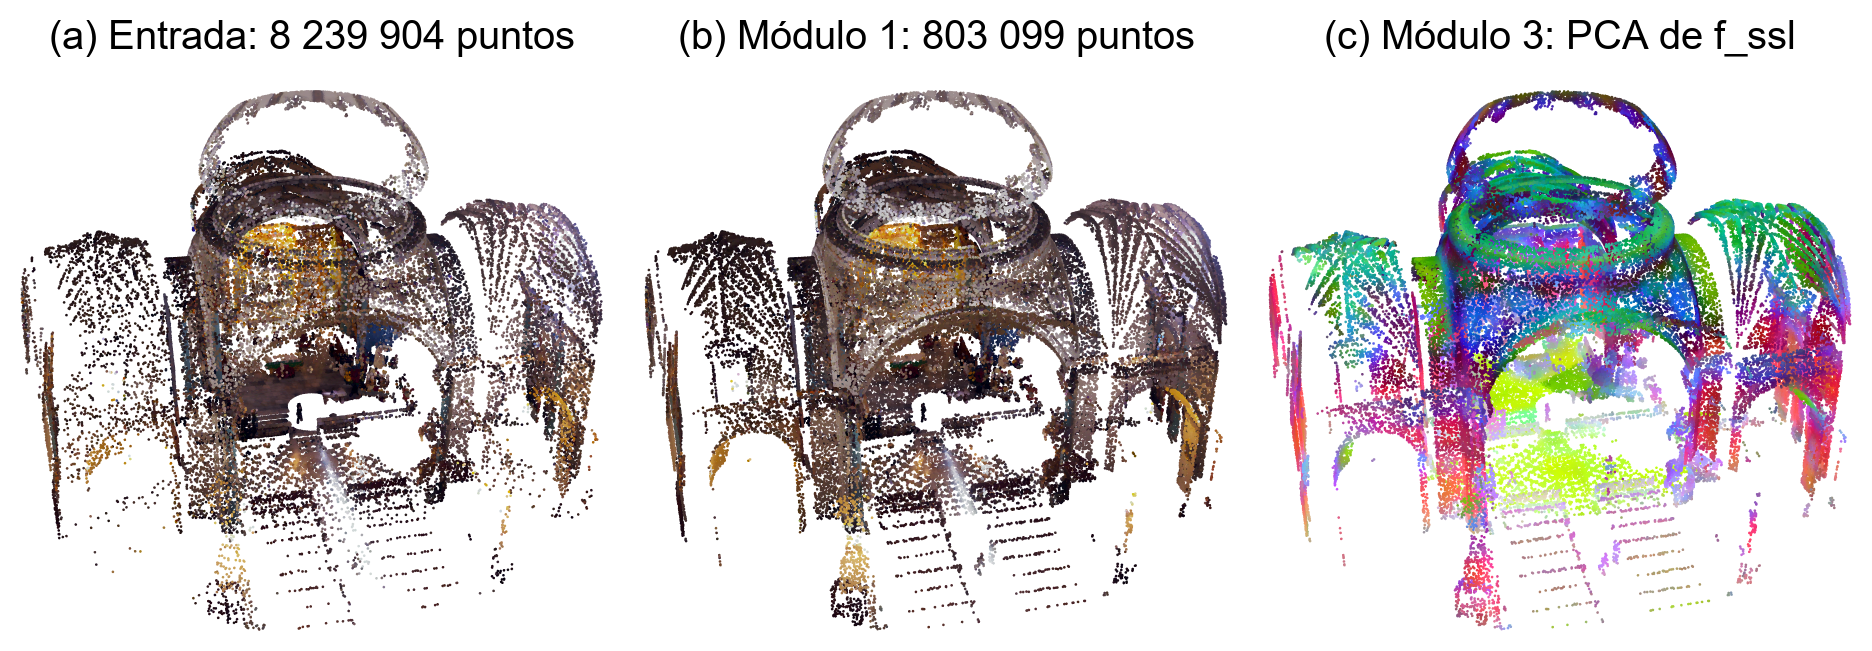
\includegraphics[width=0.8\linewidth]{imagenes/visor_pl13_entrada_m1_m3.png}
\caption[PL13 en sus tres etapas]{PL13 crudo, tras la Unidad~1 y con los descriptores de Sonata. Elaboración propia con el visor del proyecto (\hyperref[sec:anexo-software]{Anexo~A}).}
\label{fig:visor-pl13-etapas}
\end{figure}

\FloatBarrier
\subsubsection*{Paso 5. Escritura}

El contenido del archivo \texttt{.npz} está en la Tabla~\ref{tab:npz} y su
tamaño en la Tabla~\ref{tab:salidas-p2}. Tiene cinco
campos y no seis porque esta extracción se hizo antes de que el programa
guardara la semilla.

\begin{table}[!htbp]
\centering
\setstretch{1}\small
\caption[Archivo de descriptores de PL13]{Archivo de descriptores de PL13. Los campos se describen en el Paso~5 de la Sección~\ref{sec:rama-ssl}. Elaboración propia.}
\label{tab:npz}
\begin{tabular}{@{}ll@{}}
\toprule
\textbf{Campo} & \textbf{Valor en PL13} \\
\midrule
\texttt{feat} & $796\,315\times 1088$, precisión media \\
\texttt{coord} & $796\,315\times 3$ \\
\texttt{inverse} & $803\,099$ entradas \\
\texttt{grid\_size} & 0{,}02\,m \\
\texttt{n\_original} & 803\,099 \\
\bottomrule
\end{tabular}
\end{table}

\FloatBarrier
\subsubsection*{Observables\espejo{sec:observables}}
\label{sec:res-observables}

Los valores esperados y medidos están en la Tabla~\ref{tab:salidas-p2}.

\begin{table}[!htbp]
\centering
\setstretch{1}\small
\caption[Observables de Sonata en PL13: esperado y medido]{Observables de Sonata en PL13: esperado y medido. Para qué sirve cada uno se explica en la Sección~\ref{sec:observables}. Elaboración propia.}
\label{tab:salidas-p2}
\begin{tabularx}{\linewidth}{@{}>{\raggedright\arraybackslash}Xll@{}}
\toprule
\textbf{Observable} & \textbf{Esperado} & \textbf{Medido} \\
\midrule
Dimensión de $f_{\mathrm{ssl}}$ & 1088 & 1088 \\
Puntos retenidos tras el muestreo por rejilla & --- & 796\,315 de 803\,099, el 99{,}2\,\% \\
VRAM pico & Cota de 4{,}2\,GB & 34{,}60\,GB \\
Tiempo de inferencia por sección & --- & 13{,}9\,s \\
Rendimiento en puntos por segundo & --- & 57\,397 \\
Tamaño del archivo de descriptores & --- & 680\,MB \\
\bottomrule
\end{tabularx}
\end{table}

La memoria es el observable que más se aparta de lo esperado. La cota de
4{,}2\,GB se calculó para una sección de $3\times10^{5}$ puntos, y PL13 entró a
Sonata con 796\,315, unas 2{,}7 veces más, por lo que las dos cifras no se
comparan directamente. Lo que sí indica la medición es cuánto margen queda: una
sección de unos $8\times10^{5}$ puntos ocupa el 72\,\% de los 48\,GB de la GPU.
Ese es el dato con que se planificarán las secciones mayores, en lugar de la
cota.

\FloatBarrier
\subsubsection*{Revisión de los descriptores\espejo{sec:revision-descriptores}}
\label{sec:res-descriptores}

La primera vista, las
componentes principales, es el tercer panel de la
Figura~\ref{fig:visor-pl13-etapas}; las otras dos están en la
Figura~\ref{fig:sonata-pl13}, desde la misma cámara.

\begin{figure}[!htbp]
\centering
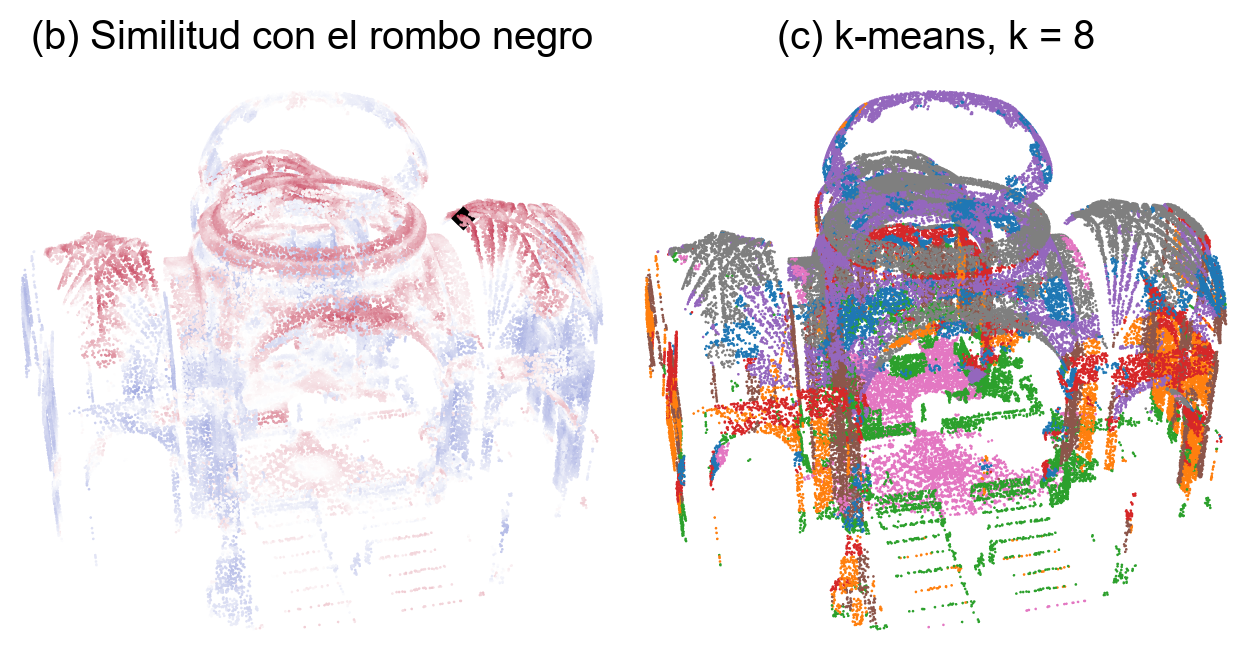
\includegraphics[width=0.6\linewidth]{imagenes/visor_pl13_descriptores_m3_sin_pca.png}
\caption[Similitud y $k$-means de los descriptores de PL13]{Similitud y $k$-means de los descriptores de PL13. Elaboración propia con el visor del proyecto (\hyperref[sec:anexo-software]{Anexo~A}).}
\label{fig:sonata-pl13}
\end{figure}

Sobre la misma muestra, las tres primeras componentes principales explican el
25{,}3\,\% de la varianza, las diez primeras el 43{,}4\,\% y el rango efectivo
es de 110{,}6 sobre 1088 dimensiones. Esto significa dos cosas. La primera es que
el color de la vista de componentes principales, que usa solo tres, muestra una
cuarta parte de la información de los descriptores; dos puntos del mismo color
pueden diferir en el resto. La segunda es que los descriptores no han colapsado:
el rango efectivo valdría 1 si todos apuntaran en la misma dirección
(Sección~\ref{sec:revision-descriptores}), y equivale aquí a unas 110
direcciones independientes.

\FloatBarrier
\subsection[Punto de Fusión]{Punto de Fusión\espejo{sec:fusion}}
\label{sec:res-fusion}

La fusión se ejecutó después de extraer y almacenar los descriptores de M2 y M3,
en CPU y con NumPy y SciPy, sin retropropagación hacia ninguno de los dos
codificadores. Sobre la capilla agrupó los puntos en unas 3\,800 regiones de
0{,}75\,m y tardó entre 68 y 80\,s. Su resultado, repetido con diez semillas,
está en la Tabla~\ref{tab:m2-m4-semillas} y en la
Figura~\ref{fig:m4-semillas}; el desglose por clase, en la
Tabla~\ref{tab:iou-clase}.

% =====================================================================
\FloatBarrier
\section[Justificación de los Parámetros del Procedimiento]{Justificación de los Parámetros del Procedimiento\espejo{sec:parametros}}
\label{sec:res-parametros}

La grilla de pruebas P0 a P5 no se ejecutó. Los valores activos se recuperaron
del código y de los registros de las corridas y se reúnen en la
Tabla~\ref{tab:res-parametros}; esa limitación se conserva en la interpretación.

\begin{table}[!htbp]
\centering
\setstretch{1}\small
\caption[Parámetros efectivos de las corridas]{Parámetros efectivos de las corridas ejecutadas. Elaboración propia a partir del código y de los registros.}
\label{tab:res-parametros}
\begin{tabularx}{\linewidth}{@{}>{\raggedright\arraybackslash}X>{\raggedright\arraybackslash}X@{}}
\toprule
\textbf{Etapa} & \textbf{Valores efectivos} \\
\midrule
M1 & Vóxel 5\,cm; $q=20$; $\lambda=2$ \\
M2, entrenamiento ArCH & 30 épocas; lote 4; 60\,000 puntos por muestra; vóxel 5\,cm; AdamW con tasa 1\,e$-$3 y mínima 1\,e$-$5, programación coseno; $\gamma=1$; $\beta=1$; DBSCAN 0{,}5\,m; semilla 0 \\
M2, pérdida y Sinkhorn & Escala 10 sobre las puntuaciones; $\epsilon_{\mathrm{sk}}=0{,}1$; $\alpha=0{,}5$, $\tau=0{,}1$, $M=8$ en la afinidad regional \\
M3 & Rejilla 2\,cm; parche 1024; sin FlashAttention; semilla 0 \\
M4 & Regiones de 0{,}75\,m; $\alpha=0{,}5$; $M=8$; $\tau=1$ con $g$ estandarizado; $\epsilon_{\mathrm{sk}}=0{,}05$; $\gamma=1$; 15 iteraciones; $K=8$; diez semillas \\
\bottomrule
\end{tabularx}
\end{table}

\FloatBarrier
\subsection[Función de Cada Paso y Efecto de Omitirlo]{Función de Cada Paso y Efecto de Omitirlo\espejo{sec:param-funcion}}

Los efectos que la Tabla~\ref{tab:funcion} atribuye a cada paso se observan en
las salidas: el descarte del filtrado en las zonas ralas (Figura~\ref{fig:m1-paso3}),
la pérdida de superficies próximas por el vóxel (Figura~\ref{fig:cubo-pl7}), las
normales ruidosas de las zonas ralas (Figura~\ref{fig:m1-paso5}) y la retención
casi total de la rejilla de Sonata (Tabla~\ref{tab:salidas-p2}).

\FloatBarrier
\subsection[Pruebas de los Parámetros]{Pruebas de los Parámetros\espejo{sec:param-criterio}}

Ninguna de las pruebas P0 a P5 se ejecutó; la elección de cada valor es la que
declara la Tabla~\ref{tab:parametros}. Lo que sí se comprobó es que la
extracción de Sonata retiene el 99{,}2\,\% de los puntos con la rejilla de 2\,cm
(Tabla~\ref{tab:salidas-p2}), de modo que el vóxel de 5\,cm del Módulo~1 es el
que fija la resolución.

\FloatBarrier
\subsection[Replicación del Procedimiento]{Replicación del Procedimiento\espejo{sec:param-replicacion}}

La replicación de la configuración de referencia está en la
Sección~\ref{sec:res-u1-repro}: el preprocesamiento dio los mismos conteos en la
laptop y en Khipu. La extracción de Sonata fija ahora una semilla y la guarda en el archivo, pero la
extracción de PL13 se hizo antes de ese cambio, de modo que su repetición exacta
no está comprobada.

% =====================================================================
\FloatBarrier
\section[Unidad 3. Entrenamiento, Calibración y Evaluación]{Unidad 3. Entrenamiento, Calibración y Evaluación\espejo{sec:unidad3}}
\label{sec:res-unidad3}

\FloatBarrier
\subsection[Procedimiento Experimental]{Procedimiento Experimental\espejo{sec:procedimiento}}
\label{sec:res-u3-proc}

\subsubsection*{E1. Diagnóstico de dominio}

El checkpoint de SemanticPOSS se aplicó primero a escenas de su propio dominio
como control positivo. La Tabla~\ref{tab:m2-control} muestra que allí funciona:
en la secuencia de validación el mIoU uno a uno es 0{,}375, casi el 0{,}384
guardado en el checkpoint, y la cabeza dominante reúne el 30\,\% de los puntos.
En la capilla, en cambio, reúne el 98{,}4\,\% y el NMI cae de 0{,}48 a 0{,}02.
Submuestrear la capilla a 80\,000 puntos, la densidad de un LiDAR, no lo corrige.
No es, entonces, un error de la extracción ni un mal checkpoint, sino una brecha
de dominio; el experimento no separa cuánto pesan el contenido, la escala y el
sensor.

\begin{table}[!htbp]
\centering
\setstretch{1}\small
\caption[Control positivo del M2 entrenado con SemanticPOSS]{M2 entrenado con SemanticPOSS (época 8) en su dominio y fuera de él. Elaboración propia a partir de los registros del experimento de dominio.}
\label{tab:m2-control}
\begin{tabular}{@{}lrrrr@{}}
\toprule
\textbf{Escena} & \textbf{Cabeza dominante} & \textbf{Cabezas $>1$\,\%} & \textbf{NMI} & \textbf{mIoU uno a uno} \\
\midrule
SemanticPOSS, validación (03) & 30{,}4\,\% & 7 & 0{,}478 & 0{,}375 \\
SemanticPOSS, entrenamiento (00) & 28{,}2\,\% & 6 & 0{,}493 & 0{,}472 \\
Capilla & 98{,}4\,\% & 1 & 0{,}018 & 0{,}114 \\
Capilla a 80\,000 puntos & 91{,}8\,\% & 4 & 0{,}033 & 0{,}099 \\
PL13 y PL7, sin etiquetas & 82{,}5 y 81{,}4\,\% & 4 & --- & --- \\
\bottomrule
\end{tabular}
\end{table}

\subsubsection*{E2. Entrenamiento con ArCH}

ArCH \cite{matrone2020benchmark} se eligió porque contiene la geometría y las
clases propias del patrimonio arquitectónico, como arcos, columnas y bóvedas,
ausentes del dominio urbano de SemanticPOSS. Se usaron 15 escenas para
entrenamiento y dos de prueba como validación; seis clases fueron conocidas
(molduras, piso, puerta/ventana, muro, escaleras y techo), tres novedosas (arco,
columna y bóveda) y \emph{other} se ignoró en la métrica principal. La
configuración está en la Tabla~\ref{tab:res-parametros}.

El mejor checkpoint alcanzó 48{,}93\,\% de mIoU de validación en la época~20 y el
de la época 30, 48{,}47\,\%. El archivo del mejor se llama
\texttt{epoch=20-step=860} y su metadato interno dice época 21; aquí se nombra por
el archivo. Es una única corrida. La Figura~\ref{fig:m2-arch-curvas} muestra que
la pérdida baja de 4{,}90 a 2{,}64 y que la validación se aplana hacia la época
20, y la Tabla~\ref{tab:m2-arch-clases}, que las clases extensas obtienen los
valores más altos y que puerta/ventana, arco y escaleras siguen siendo las más
difíciles.

\begin{table}[!htbp]
\centering
\small
\caption[IoU por clase del entrenamiento de M2 con ArCH]{IoU por clase de validación del checkpoint de M2 entrenado con ArCH (época 20). Elaboración propia.}
\label{tab:m2-arch-clases}
\begin{tabular}{lrrrrrrrrr}
\toprule
Clase & Techo & Muro & Bóveda & Piso & Columna & Moldura & Escalera & Arco & P/V \\
\midrule
IoU & .887 & .798 & .721 & .675 & .557 & .342 & .210 & .161 & .053 \\
\bottomrule
\end{tabular}
\end{table}

\begin{figure}[!htbp]
\centering
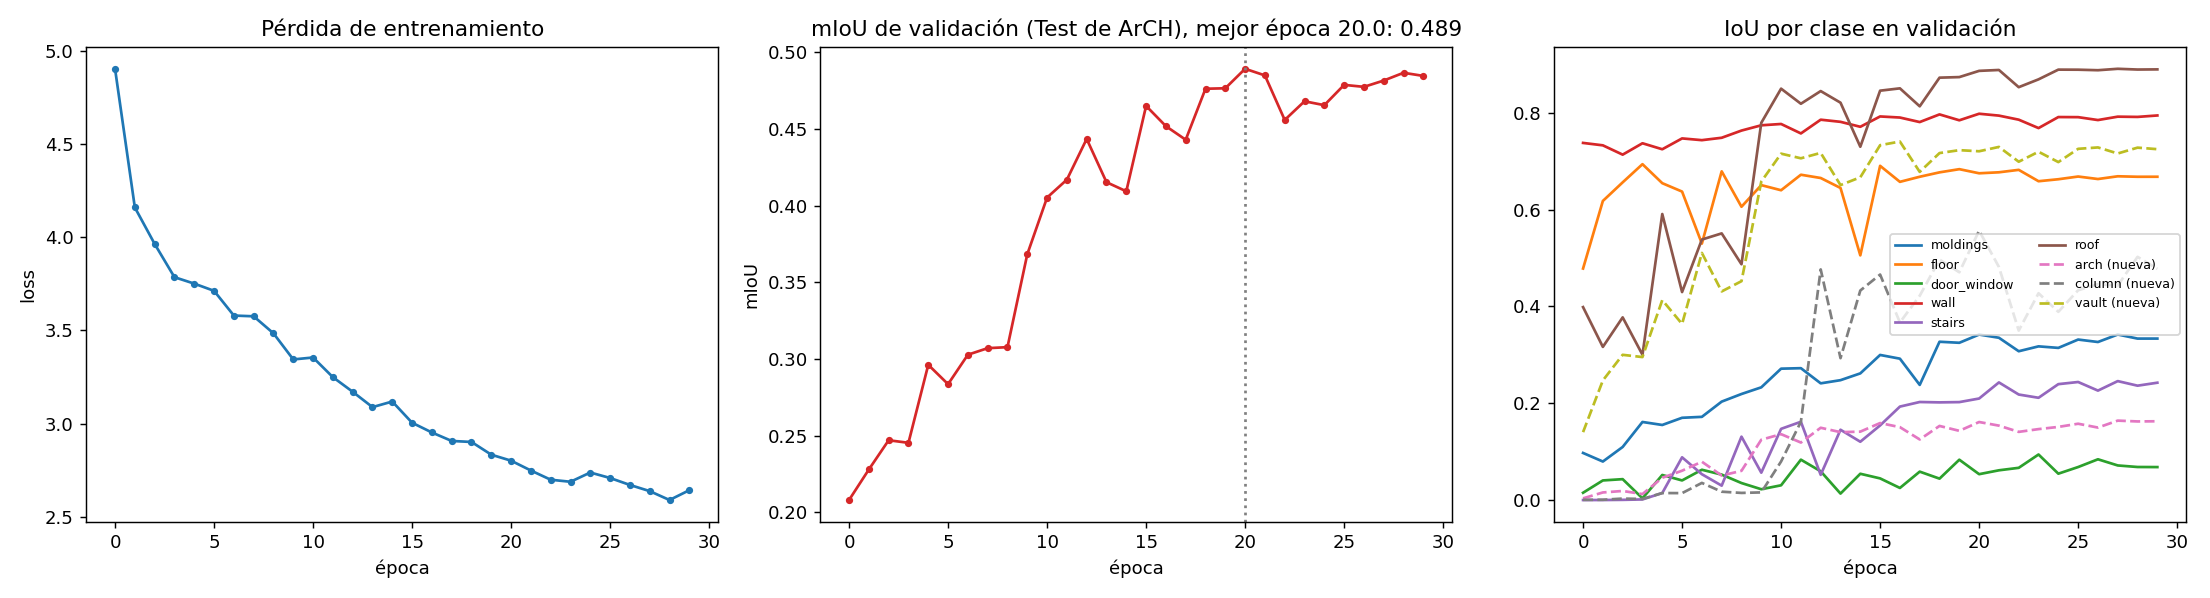
\includegraphics[width=\linewidth]{imagenes/m2_arch_curvas.png}
\caption[Curvas de entrenamiento de M2 con ArCH]{Entrenamiento de M2 con ArCH
durante 30 épocas: pérdida de entrenamiento, mIoU de validación con su mejor
época en la 20 (0,489) y IoU por clase; las clases novedosas van en línea
discontinua. Elaboración propia.}
\label{fig:m2-arch-curvas}
\end{figure}

\subsubsection*{E3. Transferencia a la capilla}

La Tabla~\ref{tab:m2-dominio} compara los tres checkpoints en la capilla. Con ArCH
la cabeza dominante baja de 98{,}4 a 44{,}5\,\% y el NMI sin \emph{other} sube de
0{,}027 a 0{,}437, y el mIoU uno a uno de 7{,}7 a 33{,}6\,\%. Los dos
checkpoints de ArCH son casi idénticos entre sí. La selección por validación
elige el de la época 20; el de la época 30 rinde 1{,}9 puntos más en la capilla,
pero esa escena no se usó para elegir, y los experimentos de fusión de las
secciones siguientes se hicieron con el de la época 30. La
Figura~\ref{fig:m2-dominio} resume los indicadores y la
Figura~\ref{fig:m2-cabeza-clase} muestra a qué cabezas va cada clase real:
SemanticPOSS manda todas a una, y ArCH reparte el techo, la pared, la cúpula y el
arco en cabezas distintas.

\begin{table}[!htbp]
\centering
\small
\caption[Transferencia de M2 a la capilla con tres checkpoints]{Transferencia de M2 a la escena de control de la Catedral de Lima. Elaboración propia a partir del resumen del experimento de dominio.}
\label{tab:m2-dominio}
\begin{tabular}{@{}lrrr@{}}
\toprule
\textbf{Métrica} & \textbf{SemanticPOSS} & \textbf{ArCH, época 20} & \textbf{ArCH, época 30} \\
\midrule
Cabeza dominante & 98,4\,\% & 44,5\,\% & 44,6\,\% \\
Cabezas con más de 1\,\% & 1 & 9 & 9 \\
NMI, todas las clases & 0,018 & 0,192 & 0,191 \\
NMI, sin \emph{other} & 0,027 & 0,437 & 0,439 \\
ARI, sin \emph{other} & 0,004 & 0,447 & 0,461 \\
mIoU uno a uno, sin \emph{other} & 7,7\,\% & 33,6\,\% & 35,5\,\% \\
\bottomrule
\end{tabular}
\end{table}

\begin{figure}[!htbp]
\centering
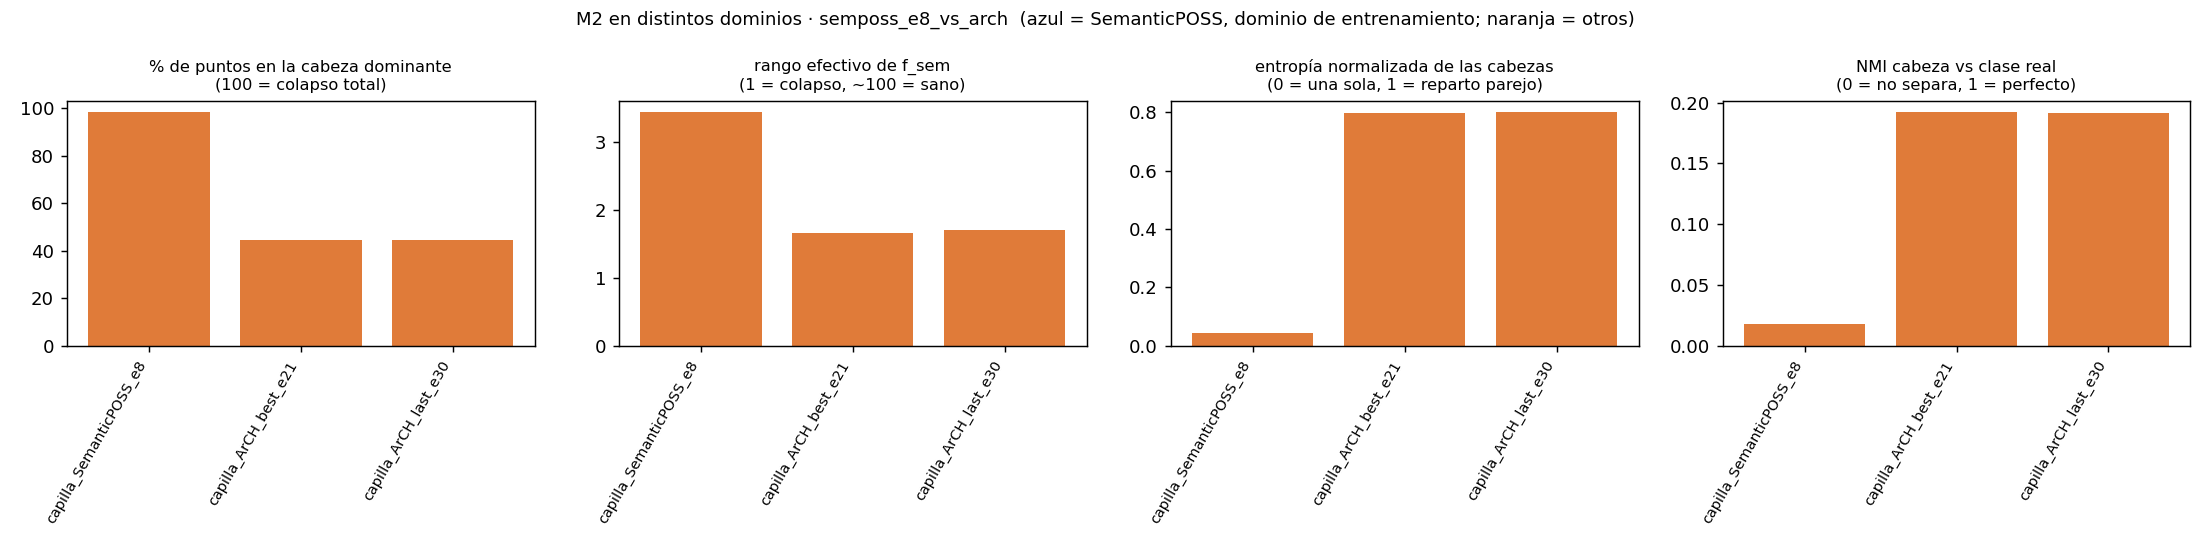
\includegraphics[width=\linewidth]{imagenes/m2_dominio_capilla.png}
\caption[Diagnóstico de dominio de M2 sobre la capilla]{Diagnóstico de dominio
de M2 sobre la escena de control: checkpoint de SemanticPOSS (época~8) frente a
los checkpoints de ArCH (épocas 20 y 30). Se reportan cabeza dominante, rango
efectivo de $f_{\mathrm{sem}}$, entropía normalizada y NMI. Elaboración propia.}
\label{fig:m2-dominio}
\end{figure}

\begin{figure}[!htbp]
\centering
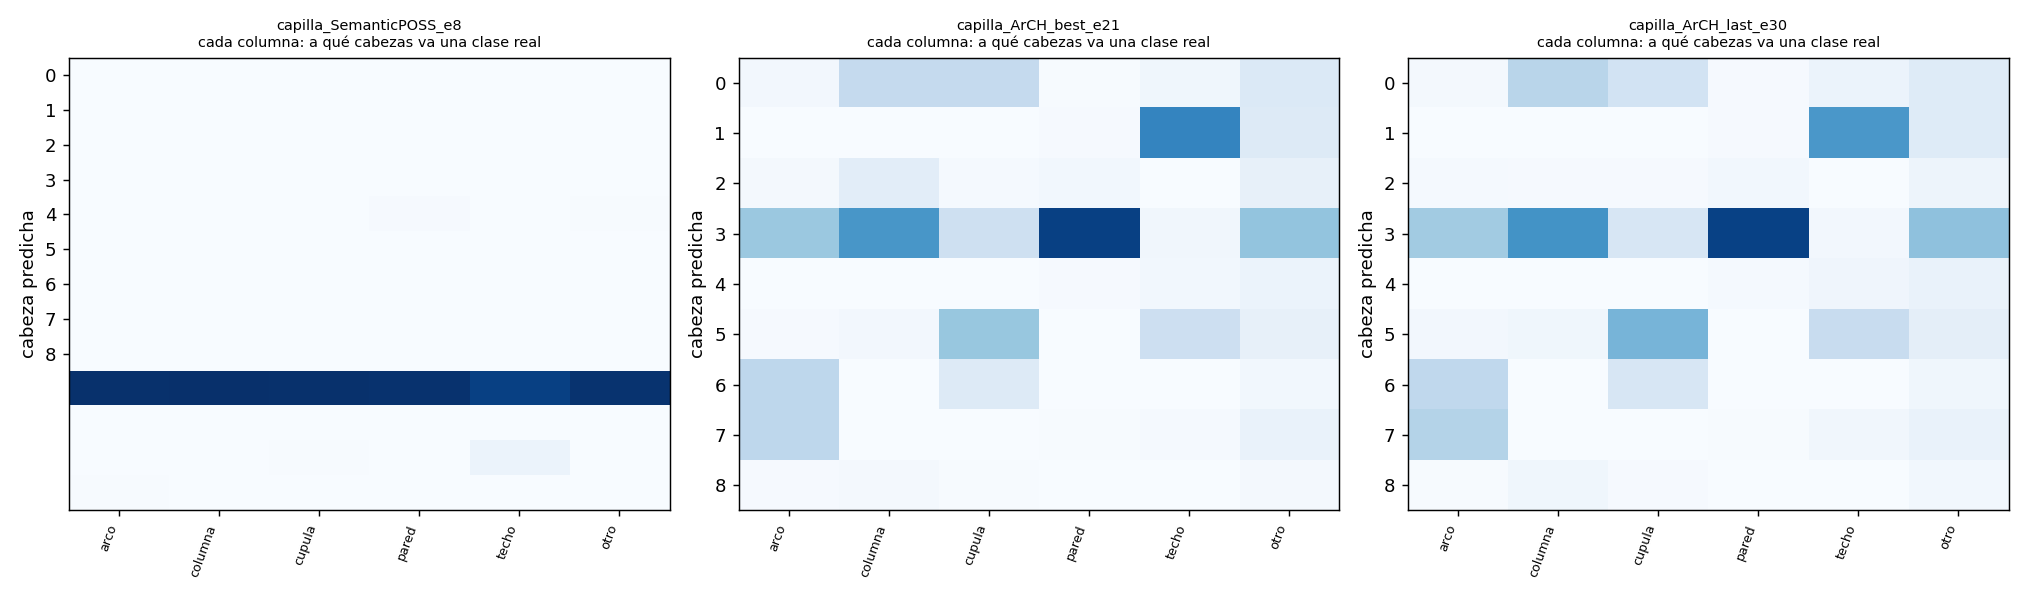
\includegraphics[width=\linewidth]{imagenes/m2_cabeza_x_clase.png}
\caption[Cabeza predicha por clase real en la capilla]{Cabeza predicha por M2 para
cada clase real de la capilla, en SemanticPOSS (época 8) y en ArCH (épocas 20 y
30). Cada columna indica a qué cabezas va una clase. El panel de SemanticPOSS
tiene 13 cabezas y rotula solo las primeras nueve. Elaboración propia.}
\label{fig:m2-cabeza-clase}
\end{figure}

\FloatBarrier
\subsection[Protocolo de Repetición]{Protocolo de Repetición\espejo{sec:repeticiones}}
\label{sec:res-u3-rep}

La comparación final se repitió con diez semillas de inicialización del
agrupamiento, con $K=8$, asignación uno a uno y sin \emph{other}. Estas
repeticiones no reentrenan ninguna red: miden la estabilidad de la etapa final,
no la de HyperNCD ni la de Sonata. La Tabla~\ref{tab:m2-m4-semillas} reúne las
cuatro combinaciones de M2 (SemanticPOSS o ArCH) y de Sonata (original o adaptado
a la Catedral) y la Figura~\ref{fig:m4-semillas} las dibuja con su mínimo y
máximo.

\begin{table}[!htbp]
\centering
\small
\caption[Resultados de M2--M4 con diez semillas]{mIoU uno a uno sin \emph{other} (\%), media $\pm$ desviación de diez semillas de agrupamiento, con $K=8$. Elaboración propia.}
\label{tab:m2-m4-semillas}
\begin{tabularx}{\linewidth}{@{}>{\raggedright\arraybackslash}Xrrrr@{}}
\toprule
\textbf{Combinación} & \textbf{M2} & \textbf{M3} & \textbf{M4 base} & \textbf{M4} \\
\midrule
SemanticPOSS + Sonata original & $35,9\pm0,6$ & $45,4\pm8,5$ & $32,5\pm0,6$ & $43,4\pm8,2$ \\
SemanticPOSS + Sonata adaptado & $35,9\pm0,6$ & $34,3\pm1,7$ & $32,5\pm0,6$ & $33,7\pm2,1$ \\
ArCH + Sonata original & $48,4\pm1,1$ & $45,4\pm8,5$ & $51,4\pm1,7$ & $52,5\pm2,5$ \\
ArCH + Sonata adaptado & $48,4\pm1,1$ & $34,3\pm1,7$ & $51,4\pm1,7$ & $47,0\pm0,8$ \\
\bottomrule
\end{tabularx}
\end{table}

\begin{figure}[!htbp]
\centering
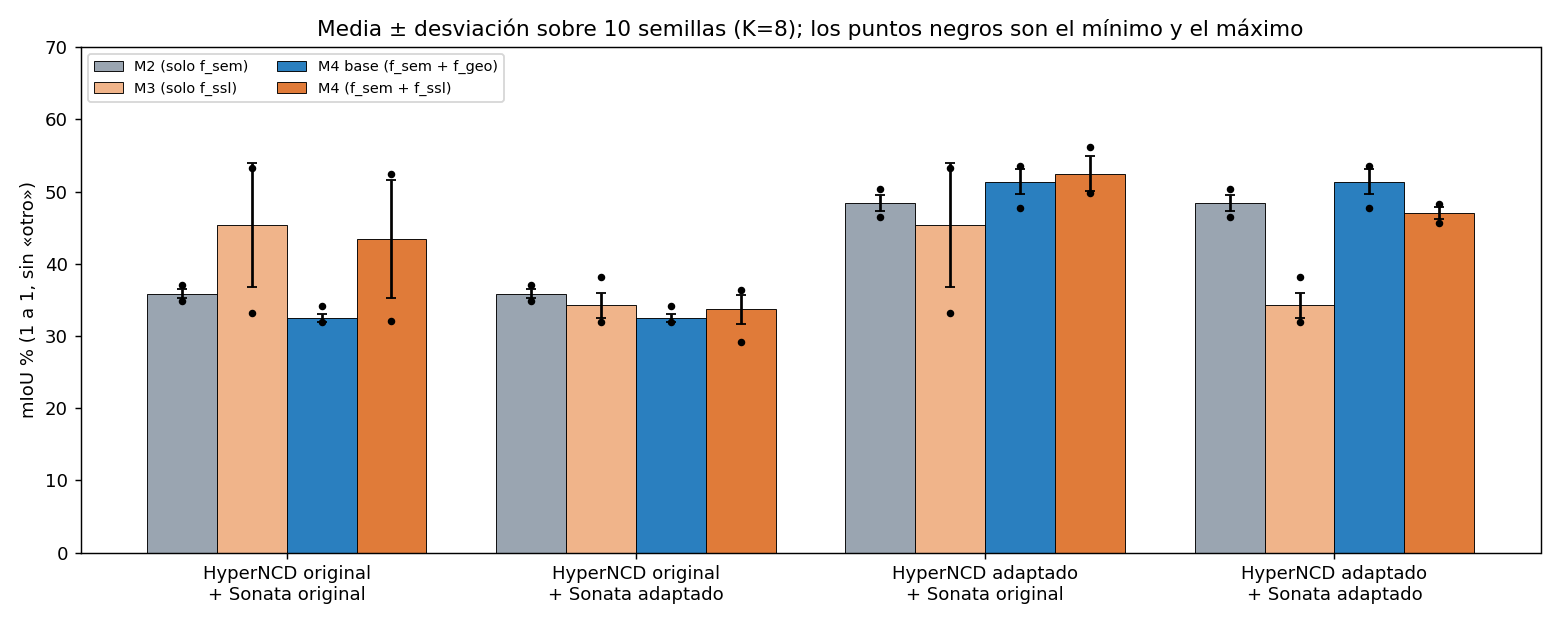
\includegraphics[width=\linewidth]{imagenes/m4_semillas.png}
\caption[Comparación M2--M4 con diez semillas y cuatro combinaciones]{mIoU uno a
uno sin \emph{other}, media y desviación de diez semillas de agrupamiento
($K=8$), para M2, M3, M4 base y M4 en las cuatro combinaciones; los puntos
negros marcan mínimo y máximo. Elaboración propia.}
\label{fig:m4-semillas}
\end{figure}

La tabla permite sustentar tres lecturas. Primera, la ganancia mayor proviene de
adaptar el dominio de M2: con ArCH, M2 sube 12{,}5 puntos (de 35,9 a 48,4), M4 base
sube 18{,}9 y M4 sube 9{,}1. Segunda, el aporte de Sonata depende del estado de
M2: cuando M2 está colapsado, la fusión M4 supera a su base en 10{,}9 puntos
(43,4 frente a 32,5), pero con M2 de ArCH la diferencia es de 1{,}1 punto (52,5
frente a 51,4), menor que las desviaciones de 1,7 y 2,5 y con rangos que se
solapan, de modo que se observa una mejora numérica, no una superioridad
demostrada. Tercera, el Sonata adaptado a la Catedral empeora: M3 baja de 45,4 a
34,3 y, con ArCH, M4 queda en 47,0, por debajo de su base. La dispersión alta de
M3 con Sonata original, de $\pm8{,}5$, indica que ese agrupamiento es inestable.

\FloatBarrier
\subsection[Trazabilidad de la Métrica]{Trazabilidad de la Métrica\espejo{sec:trazabilidad}}
\label{sec:res-u3-traza}

La Tabla~\ref{tab:iou-clase} descompone el mIoU por clase para una semilla, con
$K=8$, asignación uno a uno y sin \emph{other}; la
Figura~\ref{fig:m4-iou-clase} muestra todas las combinaciones, con y sin
\emph{other}. La clase que domina cada agregado es distinta. En M3 domina la
cúpula, con 80{,}5, mientras el arco apenas llega a 18{,}7. Con M2 de ArCH el arco
mejora (M2, 48{,}0; M4 base, 49{,}8; M4, 42{,}3), porque ArCH sí lo conoce, pero la
cúpula en M4 cae de 80{,}5 a 43{,}0: $f_{\mathrm{sem}}$ pesa más en la fusión y
separa peor la cúpula que $f_{\mathrm{ssl}}$. La columna es la más baja en todos
los métodos, entre 22 y 29. El M2 de ArCH, por tanto, no mejora todas las clases:
cambia cuáles se ganan y cuáles se pierden.

\begin{table}[!htbp]
\centering
\small
\caption[IoU por clase en la capilla]{IoU por clase (\%) en la capilla, con $K=8$, asignación uno a uno, sin \emph{other} y una semilla. M2 de ArCH (época 30). Elaboración propia.}
\label{tab:iou-clase}
\begin{tabularx}{\linewidth}{@{}>{\raggedright\arraybackslash}Xrrrrr@{}}
\toprule
\textbf{Método} & \textbf{Arco} & \textbf{Columna} & \textbf{Cúpula} & \textbf{Pared} & \textbf{Techo} \\
\midrule
M2 & 48,0 & 22,6 & 44,8 & 72,1 & 57,5 \\
M3, Sonata original & 18,7 & 28,9 & 80,5 & 68,2 & 66,4 \\
M4 base & 49,8 & 22,1 & 57,1 & 69,0 & 66,6 \\
M4, Sonata original & 42,3 & 28,6 & 43,0 & 74,2 & 65,1 \\
M4, Sonata adaptado & 27,2 & 24,3 & 43,9 & 72,0 & 69,8 \\
\bottomrule
\end{tabularx}
\end{table}

\begin{figure}[!htbp]
\centering
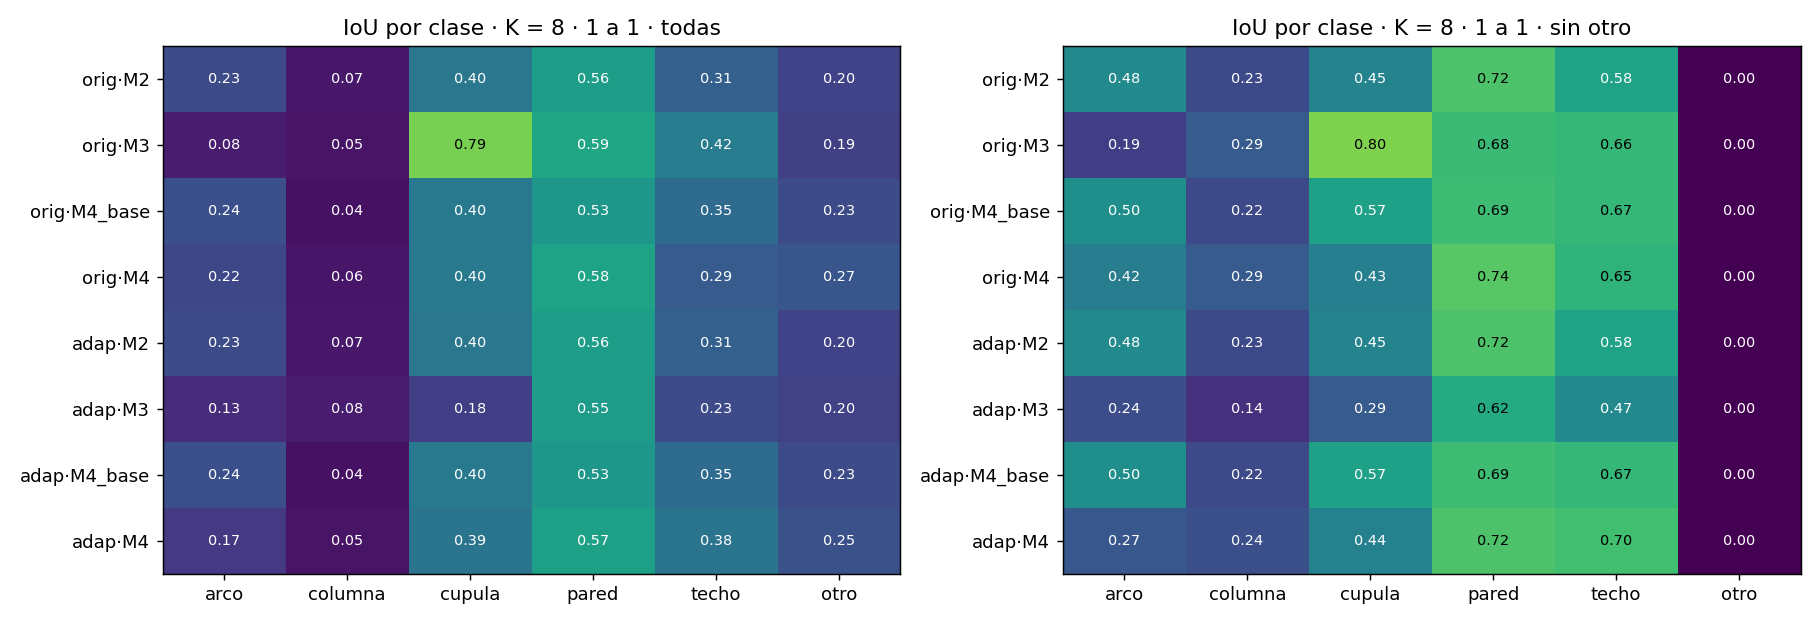
\includegraphics[width=\linewidth]{imagenes/m4_iou_por_clase.png}
\caption[IoU por clase de cada método]{IoU por clase de M2, M3, M4 base y M4 con
Sonata original (orig) y adaptado (adap), con $K=8$ y asignación uno a uno, con y
sin \emph{other}. Elaboración propia.}
\label{fig:m4-iou-clase}
\end{figure}

No se calcularon la ganancia $\Delta\mathrm{mIoU}^{\mathrm{novel}}$, la brecha
cerrada $G$ ni la sonda lineal. Las dos primeras requieren una línea base
supervisada y una separación entre clases conocidas y novedosas que la evaluación
por agrupamiento de la capilla no define, porque allí ninguna clase tiene etiqueta
de entrenamiento; la sonda lineal tiene su programa, pero no se corrió.

\FloatBarrier
\subsection[Verificación Empírica del Entorno de Cómputo]{Verificación Empírica del Entorno de Cómputo\espejo{sec:entorno-computo}}
\label{sec:res-entorno}

La Tabla~\ref{tab:res-hardware} reúne los tiempos y las memorias. El
entrenamiento de ArCH, de 30 épocas a razón de 2,5 minutos por época, usó en
promedio 62{,}8\,\% de la GPU y 74{,}7\,\% de la CPU; una prueba de una época
tardó 2{,}5 minutos con un pico de 7{,}9\,GB, y la corrida completa llegó a
9{,}5\,GB. La Figura~\ref{fig:m2-arch-recursos} muestra el uso de recursos en el
tiempo. La extracción de M2 sobre la capilla tardó 42{,}7\,s con ambos
checkpoints.

\begin{figure}[!htbp]
\centering
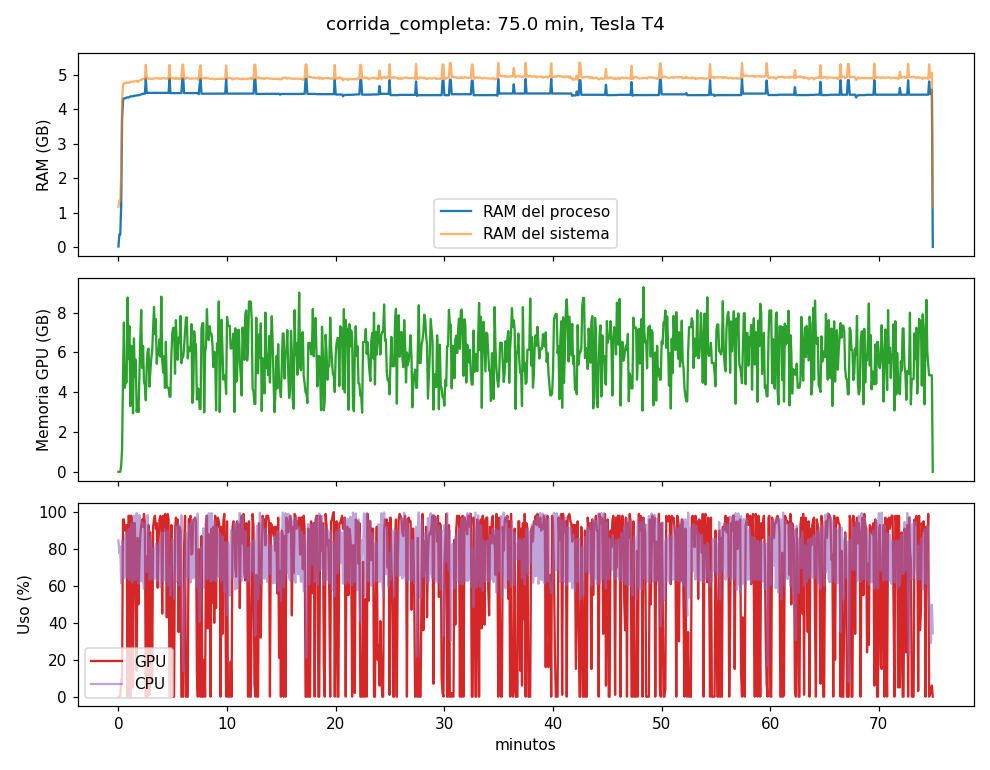
\includegraphics[width=0.9\linewidth]{imagenes/m2_arch_recursos.png}
\caption[Recursos durante el entrenamiento de M2 con ArCH]{Uso de memoria RAM,
memoria de GPU, GPU y CPU durante las 30 épocas del entrenamiento de M2 con ArCH
en una GPU T4. Elaboración propia.}
\label{fig:m2-arch-recursos}
\end{figure}

% =====================================================================
\FloatBarrier
\section[Riesgos y Mitigación]{Riesgos y Mitigación\espejo{sec:riesgos}}

\paragraph*{(i) Disponibilidad de la nube anotada.} El riesgo se materializó: los
23 archivos LAS llegaron sin etiquetas (Sección~\ref{sec:u1-datos}). Se mitigó
con la capilla etiquetada, de una sola escena, lo que limita lo que se puede
generalizar.

\paragraph*{(ii) Acceso y configuración del clúster.} Verificado: la Unidad~2
corrió en la GPU asignada (Sección~\ref{sec:res-hardware}). El entrenamiento de M2
y las evaluaciones finales corrieron en Colab.

\paragraph*{(iii) Desplazamiento de dominio.} Se materializó y se atendió con el
entrenamiento con ArCH (Sección~\ref{sec:res-u3-proc}).

% =====================================================================
\FloatBarrier
\section[Resumen de los Resultados]{Resumen de los Resultados\espejo{sec:conclusion-metodo}}

Las tres unidades produjeron las salidas declaradas por el método. El resultado
principal de M2 es que ArCH corrige el colapso de dominio del checkpoint de
SemanticPOSS y permite extraer un descriptor semántico útil para la Catedral. En
la fusión, M4 alcanza la mejor media, 52,5\,\%, pero su ventaja sobre M4 base
queda dentro de la variabilidad entre semillas, y el Sonata adaptado no mejora
al original. La evidencia es exploratoria: una escena, una corrida de
entrenamiento y diez repeticiones solo del agrupamiento.
